\documentclass{article}

% necessary for accent (linux)
\usepackage[italian]{babel}
\usepackage[utf8]{inputenc}
\usepackage[T1]{fontenc}

\usepackage{graphicx}

% to set a divider
\newcommand{\divider}{\noindent\makebox[\linewidth]{\rule{\columnwidth}{0.4pt}}}

% to count questions
\newcounter{QuestionNumber}
\newcommand{\question}{\stepcounter{QuestionNumber} {\bf Question: \arabic{QuestionNumber}}}

% path for images
\graphicspath{{./img/}}


\begin{document}
%---------------------------------------------------------------------
CAT; example

\question

NAME; square

TYPE; multi

Q; What is the area of the square?

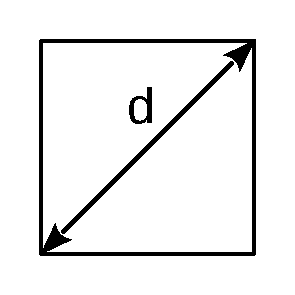
\includegraphics[width=0.3\columnwidth]{square}

DATA; $d=4\sqrt{2}\mathrm{m}$
\begin{itemize}
	\item A+100; $16\mathrm{m}$
	\item A-25; $8\mathrm{m}$
	\item A-25; $4\mathrm{m}$
	\item A-25; $32\mathrm{m}$
\end{itemize}

END;

%---------------------------------------------------------------------

\divider

%---------------------------------------------------------------------

CAT; example

\question

NAME; triangle

TYPE; true-false

Q; The figure represents a scalene triangle.

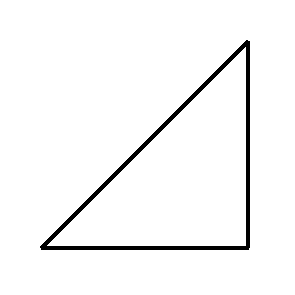
\includegraphics[width=0.3\columnwidth]{triangle}


\begin{itemize}
	\item A; false
\end{itemize}

END;

%---------------------------------------------------------------------

\divider

%---------------------------------------------------------------------
\newpage

CAT; example

\question

NAME; circle

TYPE; numerical

Q; Given the circle in figure. Compute the area in $cm^2$

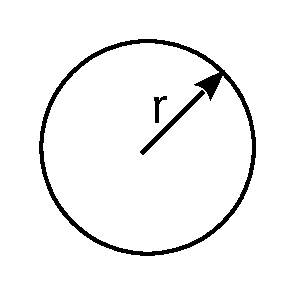
\includegraphics[width=0.3\columnwidth]{circle}

DATA; $d=2\mathrm{m}$

% Here half of the total points are given if the result
% is correct but expressed in m^2
\begin{itemize}
	\item A+100; 1973.920:0.5
	\item A+50; 19.739:0.05
\end{itemize}

END;

%---------------------------------------------------------------------

\divider

%---------------------------------------------------------------------



\end{document}